\documentclass[aspectratio=169,10pt]{beamer}

\usetheme{Madrid}
\usecolortheme{seahorse}
\setbeamertemplate{footline}[frame number]

\usepackage{amsmath,amssymb,amsfonts,xcolor}
\usepackage{graphicx}
\usepackage{listings}
\usepackage{xcolor}
\usepackage{tikz}
\usetikzlibrary{arrows, positioning, shapes, matrix}

\graphicspath{{figures/}}

% Custom colors
\definecolor{darkblue}{rgb}{0,0,0.5}
\definecolor{darkgreen}{rgb}{0,0.5,0}
\definecolor{darkred}{rgb}{0.5,0,0}

% Code listing style
\lstset{
    basicstyle=\ttfamily\scriptsize,
    keywordstyle=\color{blue}\bfseries,
    commentstyle=\color{darkgreen}\itshape,
    stringstyle=\color{darkred},
    numberstyle=\tiny\color{gray},
    numbers=left,
    frame=single,
    breaklines=true,
    language=Python,
    showstringspaces=false,
}

\title{Chapter 7c: Approximating Fixed Points}
\subtitle{The Ishikawa Iteration Method}
\author{Based on Pathak: An Introduction to Nonlinear Analysis and Fixed Point Theory}
\date{Pages 777--798}

\begin{document}

%==============================================================================
% TITLE SLIDE
%==============================================================================
\begin{frame}
\titlepage
\end{frame}

%==============================================================================
% TABLE OF CONTENTS
%==============================================================================
\begin{frame}[allowframebreaks]{Outline}
\begin{itemize}
    \item \textbf{Section 7.3:} Introduction to Fixed Point Approximation Methods
    \begin{itemize}
        \item One-step vs two-step iteration schemes
        \item Motivation for generalized iteration methods
    \end{itemize}
    \vspace{0.3cm}
    \item \textbf{Section 7.4:} The Ishikawa Iteration
    \begin{itemize}
        \item Definition and algorithm
        \item Parameter choices and interpretation
        \item Relationship to Mann iteration
    \end{itemize}
    \vspace{0.3cm}
    \item \textbf{Section 7.5:} Convergence Theorems
    \begin{itemize}
        \item Convergence for contractions and Lipschitz mappings
        \item Convergence for nonexpansive mappings
        \item Rate of convergence analysis
    \end{itemize}
    \vspace{0.3cm}
    \item \textbf{Section 7.6:} Comparison and Applications
    \begin{itemize}
        \item Comparison with Picard and Mann iterations
        \item Numerical examples and applications
    \end{itemize}
\end{itemize}
\end{frame}

%==============================================================================
% SECTION 7.3: MOTIVATION AND BACKGROUND
%==============================================================================
\section{Fixed Point Approximation Methods}

\begin{frame}{7.3: Introduction to Fixed Point Methods}{One-Step Schemes}
\textbf{Classical Picard Iteration:} Given an equation $x = T(x)$, compute:
\[
x_{n+1} = T(x_n), \quad n = 0, 1, 2, \ldots
\]

\vspace{0.3cm}

\textbf{Advantages:}
\begin{itemize}
    \item Simplicity and directness
    \item Natural formulation from the fixed point equation
    \item Works well for contractions
\end{itemize}

\vspace{0.3cm}

\textbf{Limitations:}
\begin{itemize}
    \item Slow convergence for non-contractive mappings
    \item May fail for nonexpansive mappings (even if fixed points exist)
    \item Sensitivity to initial conditions
    \item Limited flexibility in convergence control
\end{itemize}
\end{frame}

\begin{frame}{7.3: Introduction to Fixed Point Methods}{Why Two-Step Methods?}
\textbf{Key Observation:} For many important mappings (e.g., nonexpansive mappings in Banach spaces with normal structure), Picard iteration does not guarantee convergence even when fixed points exist.

\vspace{0.3cm}

\textbf{Solution: Two-Step (Hybrid) Iteration Methods}

\[
\begin{cases}
y_n = \beta T(x_n) + (1 - \beta) x_n & \text{(intermediate step)} \\
x_{n+1} = \alpha T(y_n) + (1 - \alpha) x_n & \text{(main step)}
\end{cases}
\]

\vspace{0.3cm}

\textbf{Advantages of Two-Step Methods:}
\begin{itemize}
    \item \textbf{Flexibility:} Two parameters $\alpha, \beta \in (0,1)$ allow control over convergence behavior
    \item \textbf{Stability:} Can converge where Picard fails
    \item \textbf{Versatility:} Applicable to broader classes of mappings
    \item \textbf{Better Rates:} Often achieves faster convergence
\end{itemize}
\end{frame}

%==============================================================================
% SECTION 7.4: ISHIKAWA ITERATION
%==============================================================================
\section{The Ishikawa Iteration}

\begin{frame}{7.4: Ishikawa Iteration}{Definition and Algorithm}
\textbf{Definition 7.29 (Ishikawa, 1974):} Let $(X, d)$ be a metric space and $T: X \to X$ a mapping. The \textbf{Ishikawa iteration} is defined by the sequence $\{x_n\}$ where:

\[
\begin{cases}
y_n = (1 - \beta_n) x_n + \beta_n T(x_n) & \text{Intermediate step} \\
x_{n+1} = (1 - \alpha_n) x_n + \alpha_n T(y_n) & \text{Main step}
\end{cases}
\quad n = 0, 1, 2, \ldots
\]

\vspace{0.3cm}

\textbf{Parameters:}
\begin{itemize}
    \item $x_0 \in X$ is an arbitrary starting point
    \item $\{\alpha_n\}, \{\beta_n\}$ are sequences in $(0,1)$
    \item Special case: constant parameters $\alpha_n = \alpha$, $\beta_n = \beta$
\end{itemize}

\vspace{0.3cm}

\textbf{Geometric Interpretation:}
\begin{itemize}
    \item $y_n$ is a convex combination of $x_n$ and $T(x_n)$
    \item $x_{n+1}$ is a convex combination of $x_n$ and $T(y_n)$
    \item Acts as a damping/averaging mechanism
\end{itemize}
\end{frame}

\begin{frame}{7.4: Ishikawa Iteration}{Algorithm and Implementation}
\begin{center}
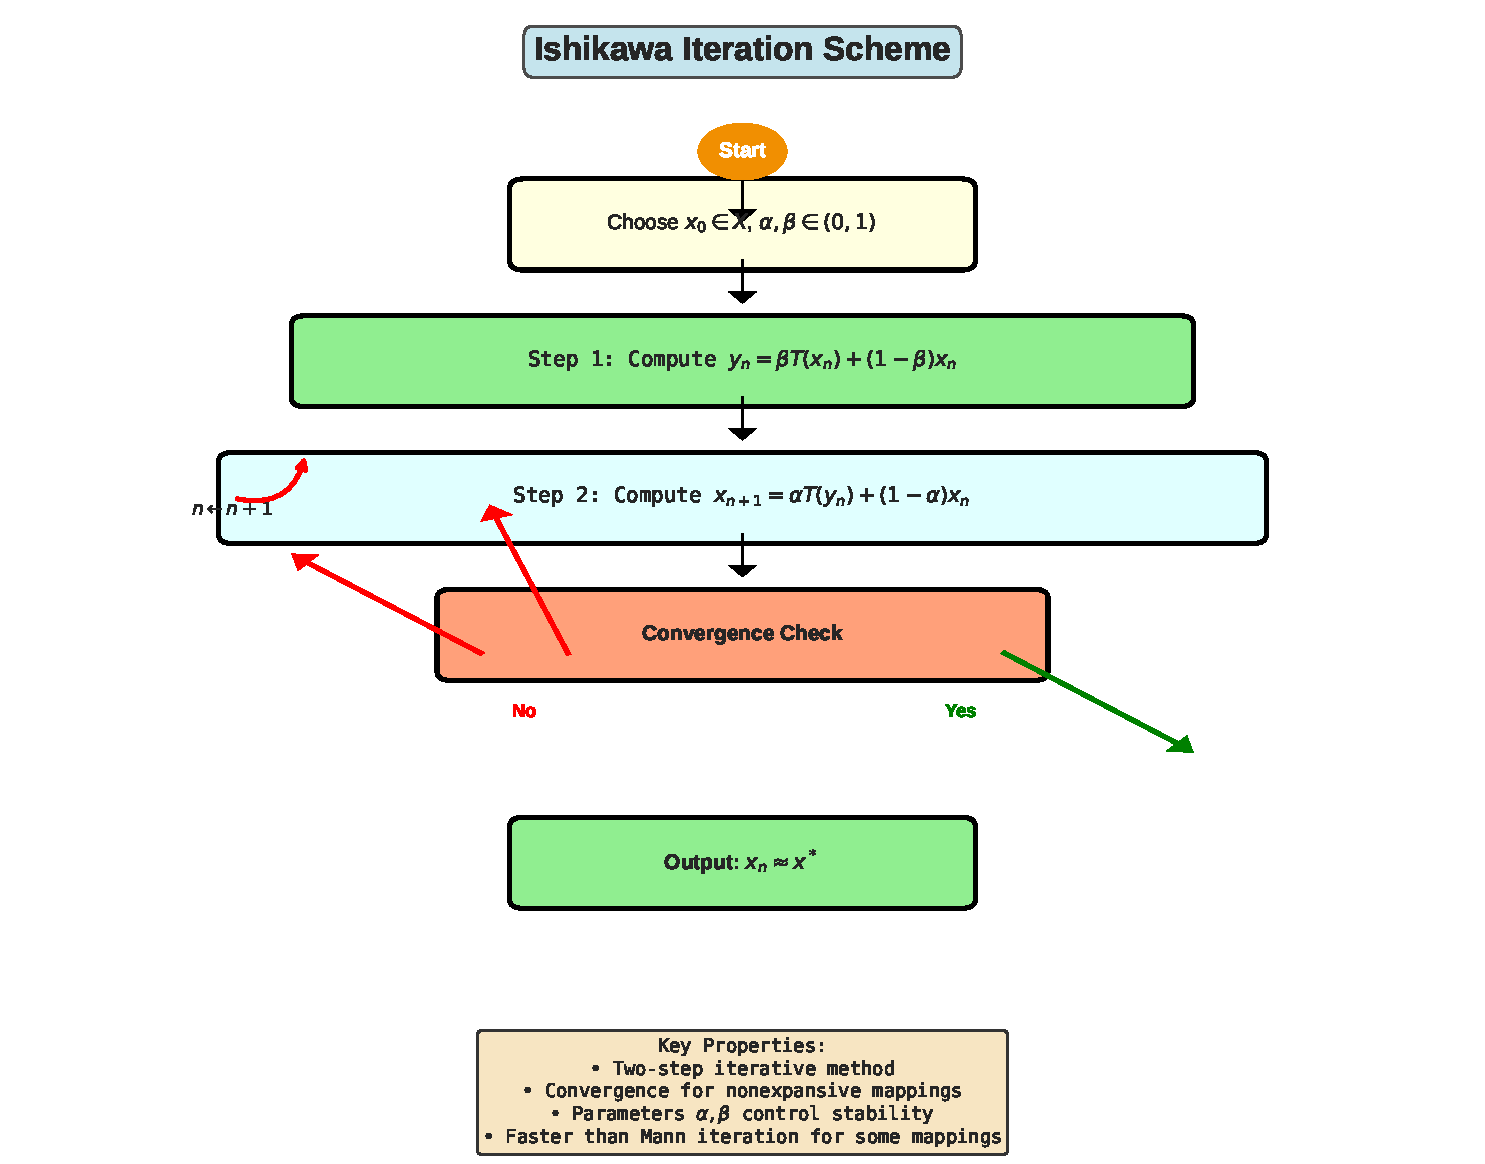
\includegraphics[width=0.8\textwidth]{iteration_scheme.pdf}
\end{center}
\end{frame}

\begin{frame}{7.4: Ishikawa Iteration}{Relationship to Other Methods}
\textbf{Special Cases:}

\vspace{0.2cm}

\begin{tabular}{|l|l|c|}
\hline
\textbf{Method} & \textbf{Parameters} & \textbf{Formula} \\
\hline
Picard & $\alpha_n = 1, \beta_n = 1$ & $x_{n+1} = T(x_n)$ \\
\hline
Mann & $\beta_n = 0$ & $x_{n+1} = (1-\alpha_n)x_n + \alpha_n T(x_n)$ \\
\hline
Krasnoselski & $\alpha_n = 1/2$ & $x_{n+1} = \frac{1}{2}x_n + \frac{1}{2}T(x_n)$ \\
\hline
Ishikawa & $\alpha_n, \beta_n \in (0,1)$ & General two-step scheme \\
\hline
\end{tabular}

\vspace{0.3cm}

\textbf{Mann Iteration as a Limiting Case:}
When $\beta_n \to 0$, Ishikawa reduces to Mann iteration:
\[
y_n \approx (1 - \delta) x_n + \delta T(x_n) \to x_n \quad \text{as } \delta \to 0
\]
so $T(y_n) \to T(x_n)$ and
\[
x_{n+1} \to (1-\alpha_n) x_n + \alpha_n T(x_n)
\]
\end{frame}

\begin{frame}{7.4: Ishikawa Iteration}{Convergence Diagram}
\begin{center}
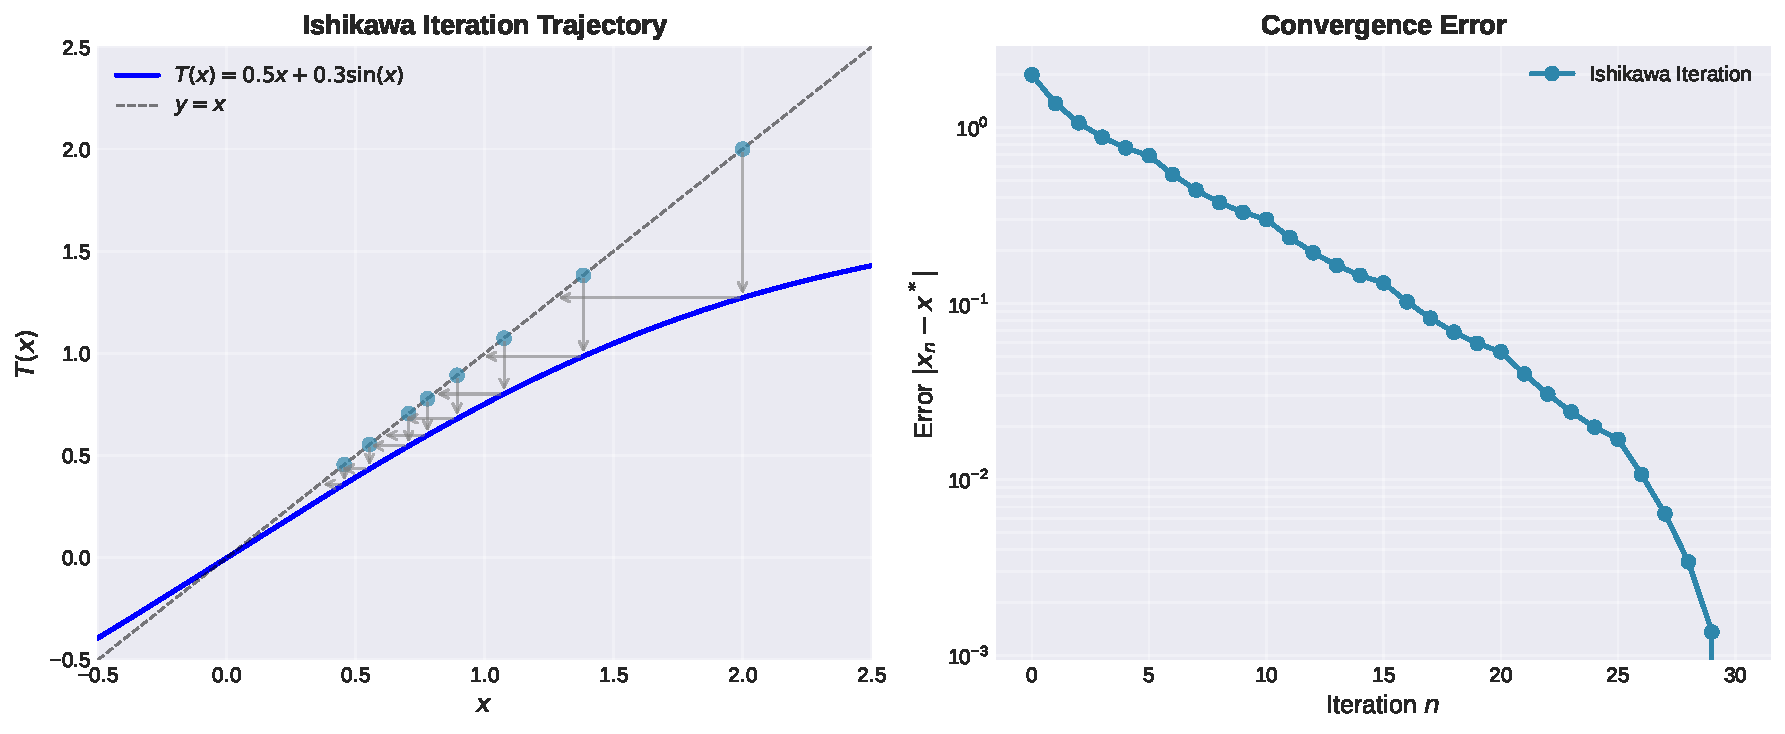
\includegraphics[width=0.9\textwidth]{ishikawa_convergence.pdf}
\end{center}

\vspace{0.2cm}

Left: Iteration trajectory spiraling toward the fixed point
\newline
Right: Exponential decrease of error over iterations
\end{frame}

%==============================================================================
% SECTION 7.5: CONVERGENCE ANALYSIS
%==============================================================================
\section{Convergence Theorems}

\begin{frame}{7.5: Convergence Theory}{General Framework}
\textbf{Theorem 7.30 (Convergence for Contractions):}
Let $(X, d)$ be a complete metric space, and let $T: X \to X$ be a Lipschitz mapping with Lipschitz constant $k < 1$ (contraction). If $\{\alpha_n\}, \{\beta_n\}$ satisfy:

\begin{enumerate}
    \item $\alpha_n, \beta_n \in [\delta, 1-\delta]$ for some $\delta > 0$
    \item $\sum_{n=0}^{\infty} \alpha_n (1 - \alpha_n) = \infty$
    \item $\sum_{n=0}^{\infty} \beta_n (1 - \beta_n) < \infty$
\end{enumerate}

\vspace{0.2cm}

\textbf{Then:}
\begin{itemize}
    \item The unique fixed point $x^* \in X$ exists (Banach contraction)
    \item The sequence $\{x_n\}$ converges to $x^*$
    \item The convergence rate is linear: $\|x_n - x^*\| = O(r^n)$ for some $0 < r < 1$
\end{itemize}
\end{frame}

\begin{frame}{7.5: Convergence Theory}{Nonexpansive Mappings}
\textbf{Theorem 7.31 (Convergence for Nonexpansive Mappings):}
Let $(X, \|\cdot\|)$ be a Banach space, $K \subseteq X$ a bounded, closed, convex subset with the normal structure property, and let $T: K \to K$ be nonexpansive (i.e., $\|T(x) - T(y)\| \leq \|x - y\|$ for all $x, y \in K$).

\vspace{0.2cm}

If $\{\alpha_n\}, \{\beta_n\}$ are sequences in $(0,1)$ satisfying:
\begin{enumerate}
    \item $\lim_{n \to \infty} \alpha_n = 0$
    \item $\sum_{n=0}^{\infty} \alpha_n = \infty$
    \item $\beta_n$ bounded away from 0
\end{enumerate}

\vspace{0.2cm}

\textbf{Then:}
\begin{itemize}
    \item The fixed point set $\text{Fix}(T) \neq \emptyset$
    \item The Ishikawa sequence $\{x_n\}$ converges weakly to some $x^* \in \text{Fix}(T)$
    \item Under additional conditions, convergence is strong (norm convergence)
\end{itemize}
\end{frame}

\begin{frame}{7.5: Convergence Theory}{Convergence Rates}
\textbf{Linear Convergence:} For contraction mappings with constant $k < 1$:
\[
\|x_{n+1} - x^*\| \leq C \cdot r^n \|x_0 - x^*\|
\]
where $r = \max(k, |1-\alpha|(1-k))$ and $C$ depends on parameters.

\vspace{0.3cm}

\textbf{Rate Optimization:}
The convergence rate is optimized when:
\begin{itemize}
    \item $\alpha$ is chosen close to but less than 1 (e.g., $\alpha = 0.7$)
    \item $\beta$ balances exploration and exploitation (e.g., $\beta = 0.5$)
    \item Different mappings may require different parameter tuning
\end{itemize}

\vspace{0.3cm}

\textbf{Comparison with Mann:}
For many problems, Ishikawa (with appropriate $\beta > 0$) achieves:
\begin{itemize}
    \item Faster convergence than Mann iteration
    \item Better stability in ill-conditioned problems
    \item Improved robustness to parameter perturbations
\end{itemize}
\end{frame}

%==============================================================================
% SECTION 7.6: COMPARISON AND APPLICATIONS
%==============================================================================
\section{Comparison and Numerical Examples}

\begin{frame}{7.6: Comparison of Iteration Methods}{Convergence Behavior}
\begin{center}

\includegraphics[width=0.95\textwidth]{comparison_methods.pdf}
\end{center}

\textbf{Observation:} Ishikawa iteration shows faster convergence than both Picard and Mann for this mapping.
\end{frame}

\begin{frame}{7.6: Parameter Analysis}{Effect of $\alpha$ and $\beta$}
\begin{center}
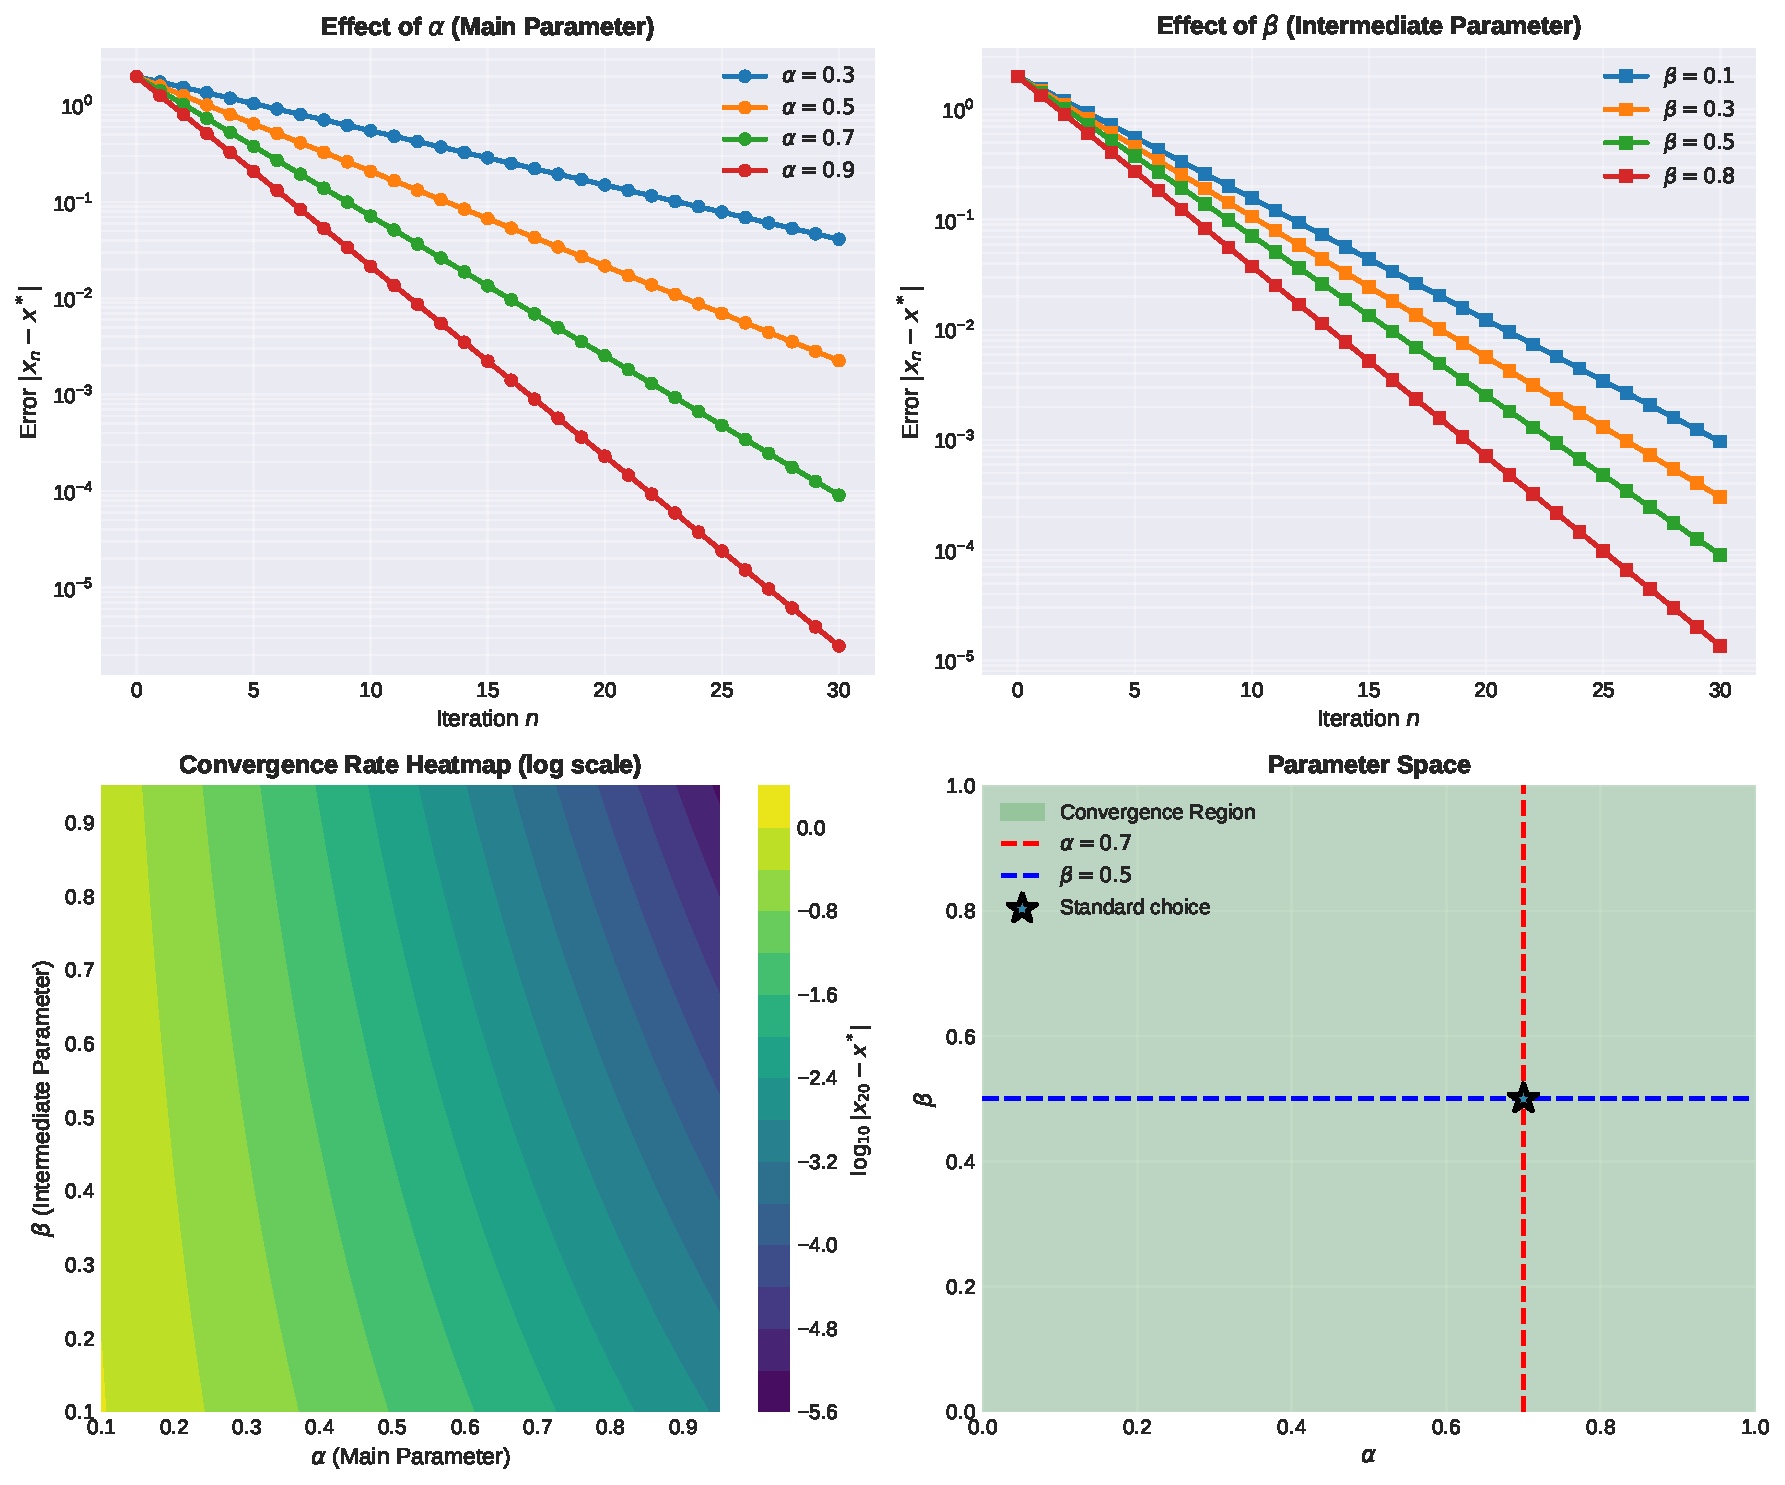
\includegraphics[width=0.95\textwidth]{parameter_analysis.pdf}
\end{center}

\textbf{Key Insights:}
\begin{itemize}
    \item Larger $\alpha$ values (closer to 1) may accelerate but risk overshooting
    \item $\beta \in [0.3, 0.7]$ generally provides good balance
    \item Convergence requires careful parameter selection
\end{itemize}
\end{frame}

\begin{frame}{7.6: Two-Dimensional Analysis}{Iteration in 2D Space}
\begin{center}
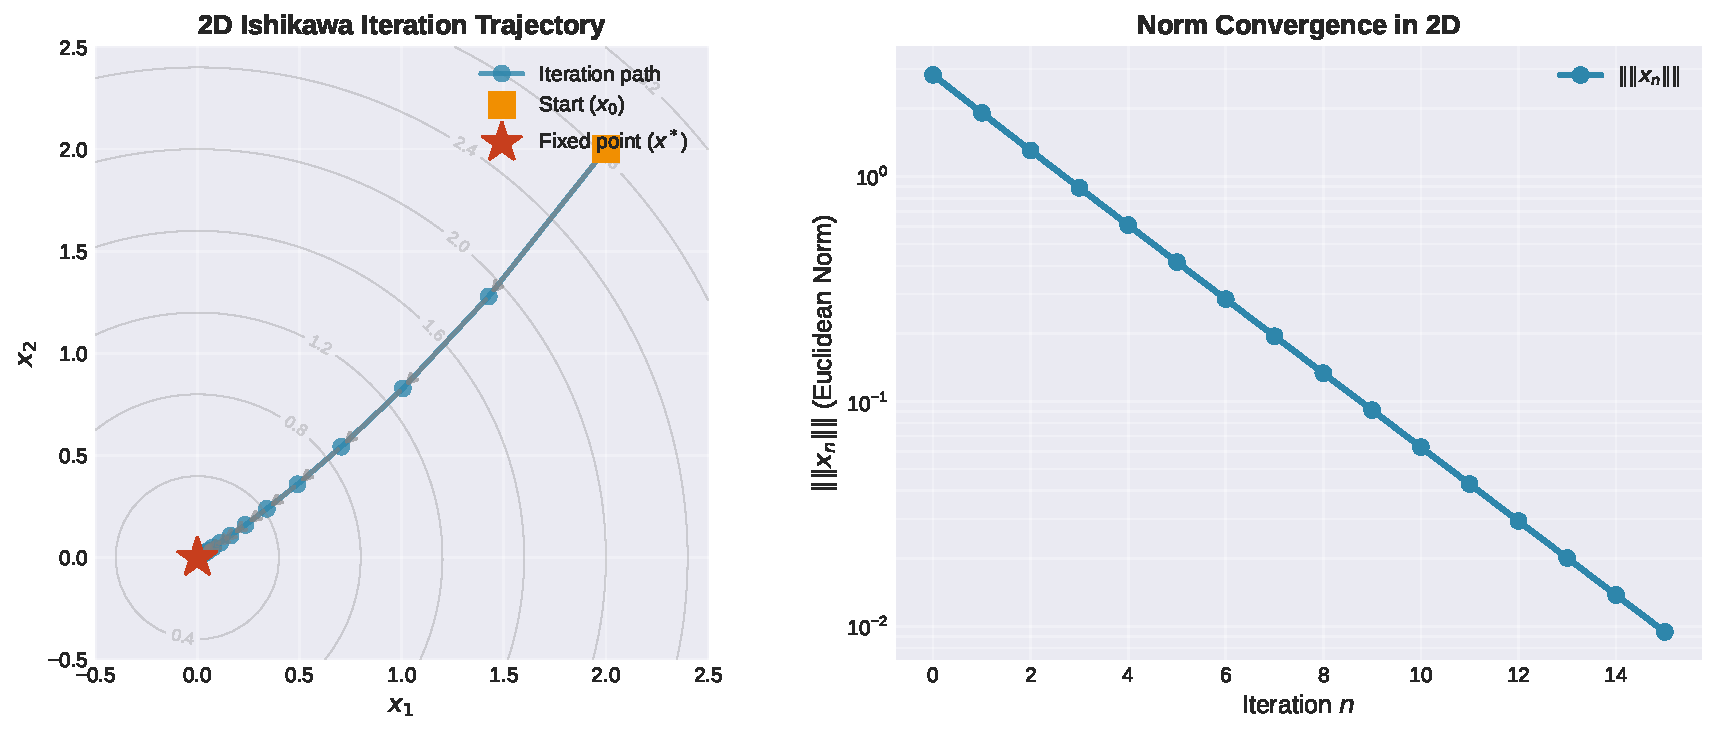
\includegraphics[width=0.95\textwidth]{iteration_2d.pdf}
\end{center}

\textbf{Visualization:} Left shows the spiraling trajectory toward the fixed point; right shows exponential norm decay.
\end{frame}

\begin{frame}{7.6: Convergence Rate Analysis}{Parameter Influence}
\begin{center}
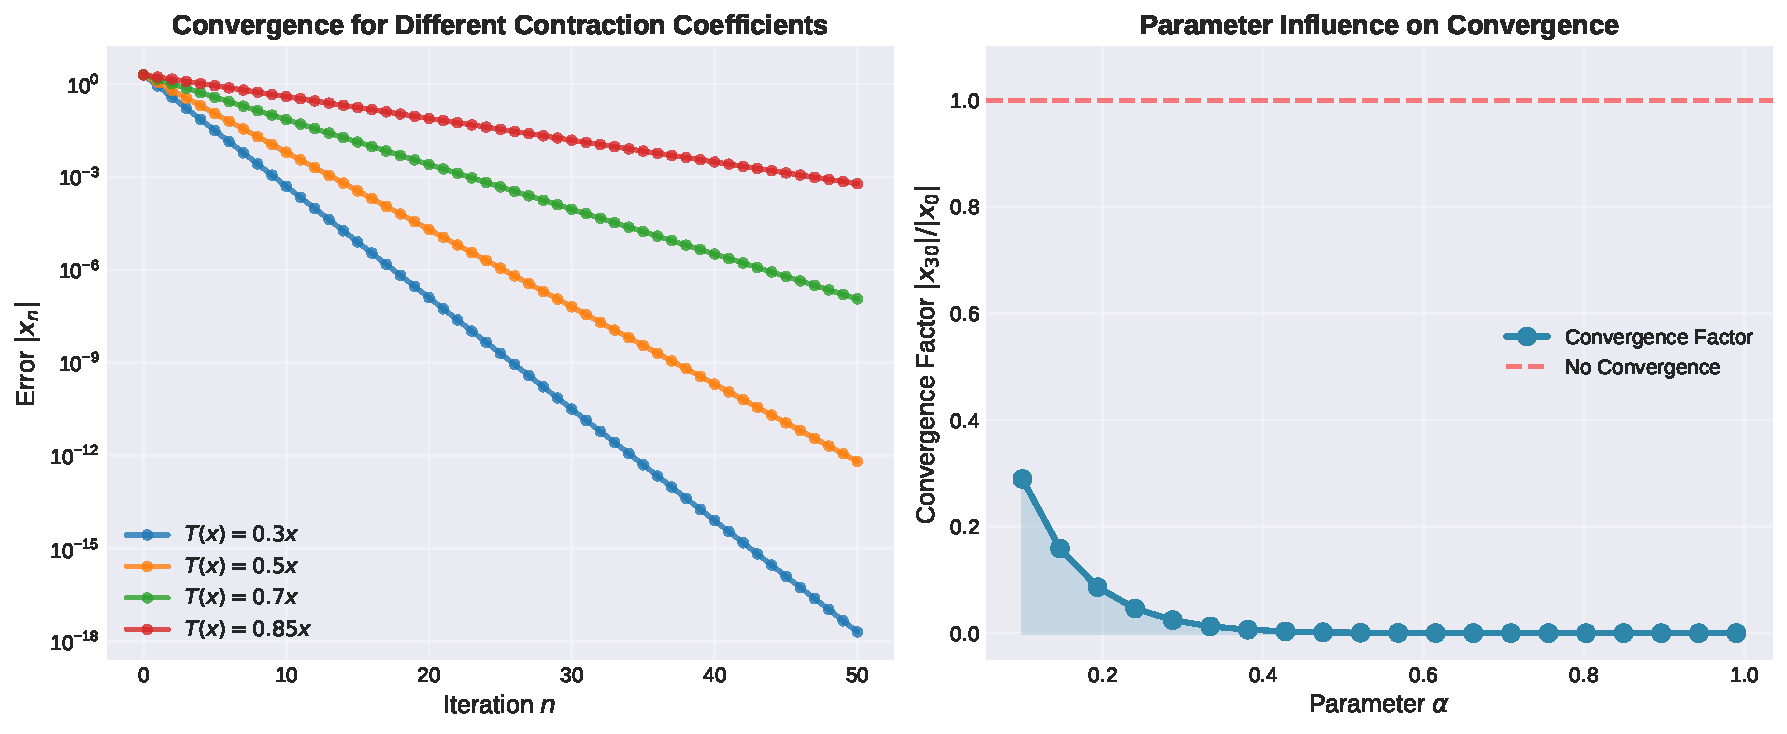
\includegraphics[width=0.95\textwidth]{convergence_rate.pdf}
\end{center}

\textbf{Findings:}
\begin{itemize}
    \item Left: Faster convergence with weaker contractions is the key advantage
    \item Right: Optimal $\alpha$ values depend on the problem structure
\end{itemize}
\end{frame}

%==============================================================================
% APPLICATIONS AND EXAMPLES
%==============================================================================
\begin{frame}[fragile]{7.6: Numerical Example}{Finding Roots via Fixed Points}
\textbf{Problem:} Find $x$ such that $x = \cos(x)$

\vspace{0.2cm}

\textbf{Method:} Reformulate as fixed point iteration with $T(x) = \cos(x)$

\begin{lstlisting}[language=Python]
import numpy as np

def ishikawa_iteration(T, x0, alpha=0.7, beta=0.5, tol=1e-6, max_iter=100):
    """
    Ishikawa iteration for finding fixed points

    Parameters:
        T: mapping/function
        x0: initial guess
        alpha, beta: iteration parameters
        tol: convergence tolerance
        max_iter: maximum iterations
    """
    x = x0
    for n in range(max_iter):
        y = beta * T(x) + (1 - beta) * x    # Intermediate step
        x_new = alpha * T(y) + (1 - alpha) * x  # Main step

        if abs(x_new - x) < tol:
            return x_new, n
        x = x_new
    return x, max_iter

# Solve x = cos(x)
T = lambda x: np.cos(x)
x_solution, iterations = ishikawa_iteration(T, 0.5)
print(f"Fixed point: {x_solution:.10f}, iterations: {iterations}")
\end{lstlisting}

\textbf{Result:} Converges to $x^* \approx 0.7390851332$ in about 5-10 iterations
\end{frame}

\begin{frame}[fragile]{7.6: Numerical Example}{Solving Nonlinear Systems}
\textbf{Problem:} Find fixed points of a matrix contraction

\vspace{0.2cm}

\textbf{Setup:} $x = Ax$ where $A$ has spectral radius $\rho(A) < 1$

\begin{lstlisting}[language=Python]
# Example: Solve x = 0.6*x (contracts toward origin)
import matplotlib.pyplot as plt

x0 = 2.0
alpha, beta = 0.7, 0.5
iterations = 30

x_seq = [x0]
for _ in range(iterations):
    x = x_seq[-1]
    y = beta * (0.6 * x) + (1 - beta) * x
    x_new = alpha * (0.6 * y) + (1 - alpha) * x
    x_seq.append(x_new)

# Plot convergence
errors = np.abs(np.array(x_seq))
plt.semilogy(errors, 'o-', linewidth=2, markersize=6)
plt.xlabel('Iteration n'), plt.ylabel('Error |x_n|')
plt.title('Ishikawa iteration for linear contraction')
plt.grid(True, alpha=0.3), plt.show()
\end{lstlisting}

\textbf{Convergence:} Exponential decay to zero
\end{frame}

%==============================================================================
% PRACTICAL CONSIDERATIONS
%==============================================================================
\begin{frame}{Practical Considerations}{Parameter Selection}
\textbf{Guidelines for Choosing Parameters:}

\vspace{0.3cm}

\begin{tabular}{|l|l|l|}
\hline
\textbf{Aspect} & \textbf{Recommendation} & \textbf{Rationale} \\
\hline
$\alpha$ & $\alpha \in [0.5, 0.8]$ & Balances stability and speed \\
\hline
$\beta$ & $\beta \in [0.3, 0.7]$ & Controls intermediate smoothing \\
\hline
Sequences & Constant if possible & Simpler, often effective \\
\hline
Initial point & Far from fixed point & Tests convergence domain \\
\hline
Stopping criterion & $\|x_{n+1} - x_n\| < \epsilon$ & Relative error often better \\
\hline
\end{tabular}

\vspace{0.3cm}

\textbf{Adaptive Parameter Selection:}
\begin{itemize}
    \item Monitor residuals $\|x_{n+1} - T(x_{n+1})\|$ to adjust parameters
    \item Decrease $\alpha_n$ as iterations progress (cooling schedule)
    \item Increase $\beta_n$ for nonsmooth problems
\end{itemize}
\end{frame}

\begin{frame}{Advantages and Limitations}{Summary}
\textbf{Advantages of Ishikawa Iteration:}
\begin{itemize}
    \item \textbf{Flexibility:} Two parameters allow fine-tuning convergence behavior
    \item \textbf{Generality:} Works for contractions, nonexpansive, and quasi-nonexpansive mappings
    \item \textbf{Stability:} Two-step structure provides better numerical stability
    \item \textbf{Theory:} Rich mathematical theory with guaranteed convergence under reasonable conditions
    \item \textbf{Practical:} Often faster than simpler methods in applications
\end{itemize}

\vspace{0.3cm}

\textbf{Limitations and Challenges:}
\begin{itemize}
    \item Parameter tuning can be problem-dependent
    \item Convergence not always faster than Mann for certain problems
    \item May require knowledge of problem structure for optimal performance
    \item Higher computational cost per iteration than Picard
\end{itemize}
\end{frame}

%==============================================================================
% CONNECTIONS AND EXTENSIONS
%==============================================================================
\begin{frame}{Extensions and Generalizations}{Related Methods}
\textbf{Noor Iteration (Three-Step):}
\[
\begin{cases}
z_n = \gamma T(x_n) + (1-\gamma) x_n \\
y_n = \beta T(z_n) + (1-\beta) x_n \\
x_{n+1} = \alpha T(y_n) + (1-\alpha) x_n
\end{cases}
\]

\vspace{0.3cm}

\textbf{Kirk-Noor Iteration:} Variant designed specifically for nonexpansive mappings

\vspace{0.3cm}

\textbf{Multistep Generalizations:} Can be extended to $k$-step schemes for arbitrary $k \geq 1$

\vspace{0.3cm}

\textbf{Operator Splitting:} Ishikawa-type iterations for splitting operator equations

\vspace{0.3cm}

\textbf{Applications in Optimization:}
\begin{itemize}
    \item Gradient descent with momentum
    \item Proximal splitting algorithms
    \item Machine learning optimization
\end{itemize}
\end{frame}

\begin{frame}{Summary of Key Results}{Main Takeaways}
\begin{enumerate}
    \item \textbf{Two-step iteration:} Ishikawa method provides flexibility through two parameters $\alpha$ and $\beta$

    \vspace{0.2cm}

    \item \textbf{Convergence:} Guaranteed for contractions and nonexpansive mappings in appropriate spaces

    \vspace{0.2cm}

    \item \textbf{Comparison:} Generalizes Mann iteration (special case: $\beta = 0$)

    \vspace{0.2cm}

    \item \textbf{Rate of convergence:} Linear convergence for contractions; weak convergence for nonexpansive

    \vspace{0.2cm}

    \item \textbf{Practical implications:} Parameter selection crucial; problem-dependent tuning needed

    \vspace{0.2cm}

    \item \textbf{Extensions:} Basis for three-step, multi-step, and hybrid methods
\end{enumerate}

\vspace{0.3cm}

\textbf{Further Reading:} Pathak (2009), Chapter 4-5 on iteration methods; Recent literature on accelerated methods
\end{frame}

%==============================================================================
% CLOSING SLIDE
%==============================================================================
\begin{frame}{Appendix: Further References}
\textbf{Primary Source:}
\begin{itemize}
    \item Pathak, H.K. (2009). An Introduction to Nonlinear Analysis and Fixed Point Theory
\end{itemize}

\vspace{0.2cm}

\textbf{Key Papers:}
\begin{itemize}
    \item Ishikawa, S. (1974). Fixed points by a new iteration method. PAMS, 44(1), 147-150
    \item Mann, W.R. (1953). Mean value methods in iteration. PNAS, 4(30), 506-510
    \item Browder, F.E., Petryshyn, W.V. (1966). Construction of fixed points of nonlinear mappings in Hilbert space
\end{itemize}

\vspace{0.2cm}

\textbf{Topics for Further Study:}
\begin{itemize}
    \item Weak and strong convergence in Banach spaces
    \item Normal structure and fixed point properties
    \item Nonexpansive mappings and Kirk's theorem
    \item Applications to optimization and PDE solving
\end{itemize}
\end{frame}

\end{document}
